\documentclass[]{scrartcl}
\usepackage{../template/Preamble}

\setcounter{section}{1}
\newcommand{\exercise}{Exercise \thesection}
\newcommand{\duedate}{2020-11-16, 23:59}

\begin{document}
\section*{\exercise}
\subsection{Reading}
\subsection{Moore's Law}
\subsubsection{}
Apply Moore's Law to currently fastest Supercomputer to extrapolate time until exa
scale performance is achieved.
\begin{enumerate}
	\item Consider derived law stating that computing power doubles every 18 months:
	\begin{equation}
		P_{\textrm{compute}}(t) = N_0 2^{\frac{1}{18} t}
	\end{equation}
	where $ N_0 $ is the computing power at time 0 and $ t $ the time in months.
	\item Set $ P_{\textrm{compute}} $ to \SI{1e18}{flop\per\second}.
	\item Set $ N_0 $ to current max performance of \SI{415530e12}{flop\per\second}
	(\emph{Supercomputer Fugaku})\footnote{https://top500.org/lists/top500/2020/06/}.
\item Solving for $ t $ yields a time of $ \approx23 $ months (see figure~\ref{fig:Moore}).
\end{enumerate}
$ \Rightarrow $ extrapolating from current performance using a derived Moore's law
Exa scale computing power will be achieved in approximately 23 months or almost two years.
\begin{figure}[htpb]
	\centering
	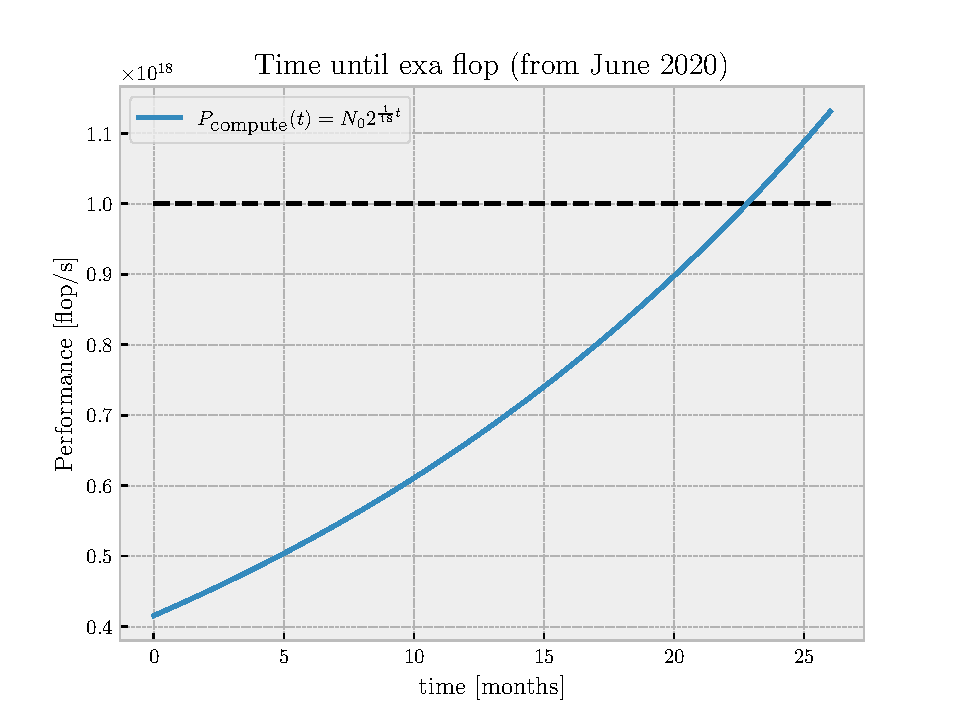
\includegraphics[width=0.8\linewidth]{./plots/Moore}
	\caption{Extrapolating time until exaflop from derived Moore's law}%
	\label{fig:Moore}
\end{figure}
\subsubsection{}
Determine time until exa scale from growth rate from TOP500 list
\begin{enumerate}
	\item Use data from 2007 and 2011
	\item Linear fit (on log scale) yields that exaflop performance should
		have been reached around 2018 (see figure~\ref{fig:GrowthRate})
\end{enumerate}
\begin{figure}[htpb]
	\centering
	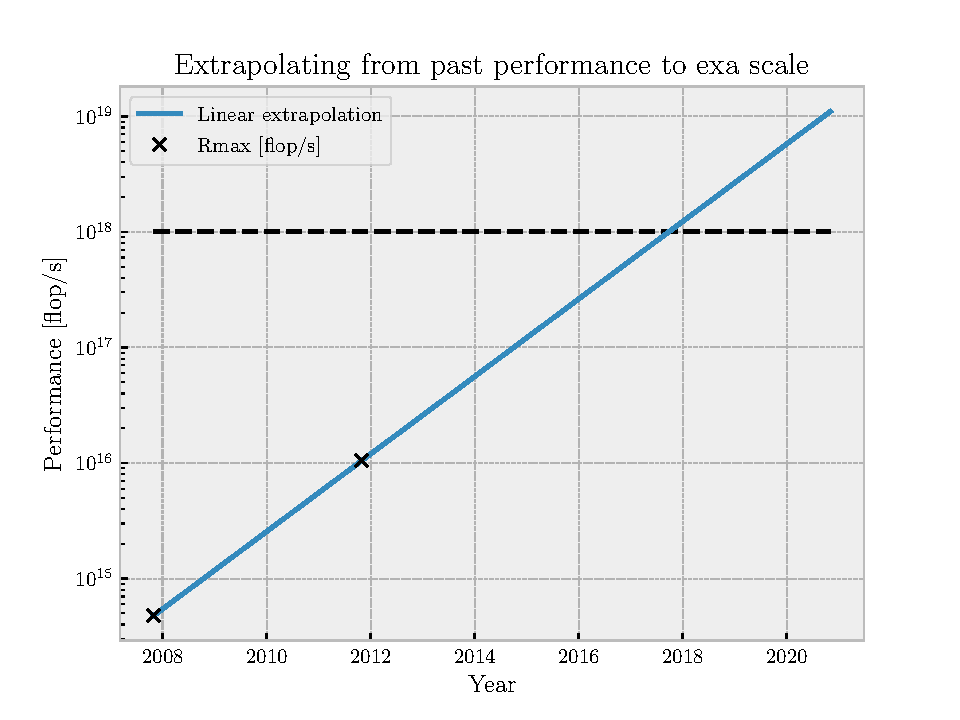
\includegraphics[width=0.8\linewidth]{./plots/GrowthRate.pdf}
	\caption{Extrapolating time until exaflop from TOP500 data using linear fit}%
	\label{fig:GrowthRate}
\end{figure}
$ \Rightarrow $ Extrapolating from past performance exaflop performance should have been
achieved around 2018, which is evidently not the case. Note however that extrapolation
from two data points is not very robust.

\newpage
\subsection{Amdahl's Law}
\subsubsection{}
\begin{itemize}
    \item new CPU 10 times faster
    \item old CPU spent 40\% of execution time on calculations
    \item remaining time was for IO
\end{itemize}
\begin{align}
    S &:= 60\%\\
    P &:= 40\%\\
    N &:= 10\\\nonumber\\
    Speedup &= \frac{1}{.6+\frac{.4}{10}} = 1.563
\end{align}

$\Rightarrow$ We would expect a 56\% performance improvement from the new CPU\@.

\subsubsection{}
\begin{itemize}
    \item 20\% of compute time is used for squaere roots
    \item possibilities:
        \begin{itemize}
            \item improve floating point square root calculations by factor of 10
            \item improve all fp operations by 1.6
        \end{itemize}
    \item 50\% of operation is spent on FP
\end{itemize}
\begin{align}
    S_1 &= \frac{1}{(1-(0.5\cdot 0.2))+\frac{0.5\cdot0.2}{10}}\\
        &= 1.099\\\nonumber\\
    S_2 &= \frac{1}{(1-0.5)+\frac{0.5}{1.6}}\\
        &= 1.231
\end{align}
$\Rightarrow$ By accelerating all FP operations by a facctor of 1.6 a speedup of 23\% can be observed and therefore is the optimal solution (in contrast to only 9.9\% when only speeding up FPSQRT).

\subsubsection{}
\begin{align}
    100 &= \frac{1}{(1-P)+\frac{P}{128}}\\
    \Leftrightarrow P&= 0.9978\\
    \Rightarrow S &\leq 0.22\%
\end{align}
\end{document}
